% !TEX root = ../intro-stellar-physics.tex

We now have almost all of the physics necessary to describe the lift of a star. The nuclear physics enters in an equation for the luminosity, which we shall derive next. We then need to discuss departures from the classical ideal gas equation of state; this becomes important for low-mass stars and sets the minimum stellar mass.

\section{The luminosity equation}

We've established the relations for the enclosed mass,
\begin{equation}\label{e.mass}
\DD{m}{r} = 4\pi r^{2}\rho,
\end{equation}
the pressure,
\begin{equation}\label{e.pressure}
\DD{P}{r} = -\rho\frac{Gm}{r^{2}},
\end{equation}
and the temperature,
\begin{eqnarray}\label{e.temperature-radiative}
\DD{T}{r} &=& - \frac{L}{4\pi r^{2}}\frac{3\rho\kappa}{4ac T^{3}}\qquad \textrm{in radiative regions;} \\ 
\label{e.temperature-convective}
\DD{T}{r} &=& \frac{T}{P}\tderiv{\ln T}{\ln P}{S}\DD{P}{r} \quad \textrm{in convective regions}.
\end{eqnarray}
We need an equation for the luminosity $L(r)$, which we now derive.

\begin{marginfigure}
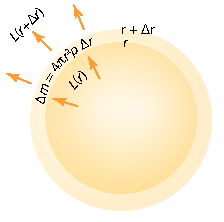
\includegraphics[width=\linewidth]{luminosity-eqn}
\caption[Heat balance in a mass shell]{Heat balance in a shell $\Delta m$.}
\label{f.luminosity}
\end{marginfigure}
Suppose we have a shell of mass $\Delta m$ lying between surfaces $r$ and $r+\Delta r$ (Fig.~\ref{f.luminosity}). The shell gains heat from nuclear reactions at a rate $\Delta m \times \varepsilon$, where $\varepsilon$ is the heating rate per unit mass.  In addition, there is heat entering the shell from below at a rate $L(r)$ and heat leaving the top of the shell at a rate $-L(r+\Delta r)$.
If the shell is neither gaining or losing heat, then these terms must balance:
\[ 4\pi r^{2}\rho\varepsilon\,\Delta r + L(r) - L(r+\Delta r) = 0. \]
This reduces to our fourth equation of stellar structure,
\begin{equation}
\label{e.luminosity}
\DD{L}{r} = 4\pi r^{2}\rho\varepsilon.
\end{equation}
These equations are supplemented by an equation of state $P = P(\rho,T)$.

\section{Contraction to the main sequence}
\label{s.contraction-to-main-sequence}
When the core is too cool for nuclear reactions to power the luminosity from the surface (remember, the luminosity is set by the mass of the star and its opacity) then the star must contract.\marginnote{When the radius is changing, an extra term appears in eq.~(\ref{e.luminosity}) giving the luminosity evolved from gravitational contraction.}

\subsection{Degeneracy}
\label{s.degeneracy}

As a star contracts, the particles within it are packed ever closer together.  As we saw from our discussion of ionization, the behavior of particles must change when the separation between particles is of the order of the uncertainty in their positions.  Equivalently, our classical description breaks down when the particle density exceeds roughly
\begin{equation}\label{e.heuristic-quantum-density}
    \frac{1\;\textrm{particle}}{(\Delta x)^3} 
    = \left(\frac{\Delta p}{h}\right)^3 
    \sim \left(\frac{m\kB T}{h^2}\right)^{3/2}.
\end{equation}
Another way to put this is that quantum effects become important when there is roughly 1 particle in a normalized phase space volume $\dif^{3}x\,\dif^{3}p/h^{3}$.

Suppose we have two identical particles in a quantum state. Since the particles are identical, if we exchange them the wavefunction can only change by a phase factor\sidenote{See Box~\ref{sb.identical-particles}} $e^{i\delta}$. If we exchange the particles again, we are back to our original state; as a result, $e^{2i\delta} = 1$, and therefore $\delta = 0$ or $\pi$. Hence upon the exchange of particles, the wavefunction either is unchanged ($\delta=0$) or it changes sign ($e^{i\pi}=-1$).
\begin{quote}\itshape
    There are two types of particles in this world: those that change sign under exchange; and those that don't.
\end{quote}
Particles that don't change sign under exchange are called \newterm{bosons} and have integer spin. Photons are bosons. Particles that change sign under exchange are called \newterm{fermions} and have half-integer spin. Electrons, neutrinos, protons, and neutrons are all fermions. 

A consequence of the fermion wavefunction changing sign when any two particles are exchanged is that the wavefunction vanishes if any two particles are in the same state---that is, they have the same position, momentum, and spin. For spin-half particles like electrons, then means we can put at most two such electrons in the same position and momentum state; we do this by having their spins antiparallel.

\begin{sidebar}[Identical Particles]
\label{sb.identical-particles}
To understand how the interchange of identical particles works in more detail, let's start by recalling some features of quantum mechanics. This discussion is based on the treatment of \citet{Feynman1989The-Feynman-Lec}.
We denote a state as $\ket{a}$, where $a$ is just a label.  For example, $a$ could be "electron with such-and-such momentum".  The probability of finding the electron in some other state $\phi$ is given by $|\braket{\phi}{a}|^2$, where $\braket{\phi}{a}$ is a complex number known as the probability amplitude.

Now suppose we have two particles, a and b, and we scatter them so that one particle ends up in detector 1 and the other ends up in detector 2. There are two ways this can go, as shown here.
\begin{center}
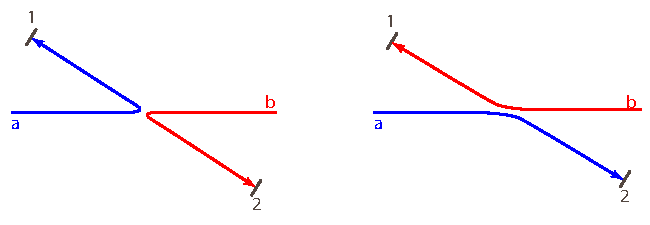
\includegraphics[width=\linewidth]{scattering-classical}
\end{center}
Classically, we would argue that the probability of getting either particle in detector 1 is just
\begin{equation}
    \mathcal{P}(\textrm{a or b in 1}) = \mathcal{P}(\textrm{a in 1}) + \mathcal{P}(\textrm{b in 1}).
\end{equation}
If particles a and b are different---e.g., one is a \carbon\ nucleus and the other is an \oxygen\ nucleus---then this holds in quantum mechanics as well. Quantum mechanically, we write
\begin{equation}
    \mathcal{P}(\textrm{a or b in 1}) = |\braket{1}{a}\braket{2}{b}|^2 + |\braket{2}{a}\braket{1}{b}|^2.
\end{equation}
If the particles are identical, however---for example, if a and b are two electrons with identical spin---then this picture is wrong.

Because of the uncertainty principle, we cannot follow the trajectories of a and b with infinite precision to see which is which; instead, the situation is more analogous to the depiction shown here.
\begin{center}
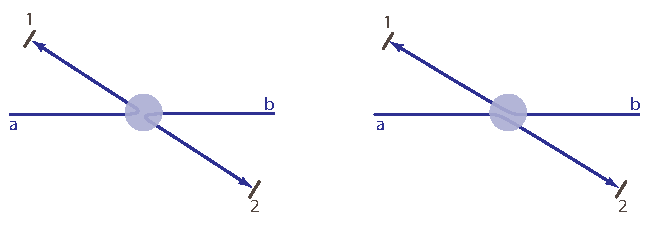
\includegraphics[width=\linewidth]{scattering-quantum}
\end{center}
There are now two indistinguishable ways of arriving at the final state---in this case, an electron in detector 1 and an electron in detector 2. According to quantum mechanics, we must therefore sum the amplitudes for getting to the final state, \emph{before taking the square}. That is, the probability for this one particle to end up in detector 1 and the other to end up in detector 2 is
\begin{eqnarray}
    \mathcal{P}(\textrm{a or b in 1}) &=& |\braket{1}{a}\braket{2}{b} + \braket{2}{a}\braket{1}{b}|^2\nonumber\\
    &=& |\braket{1}{a}\braket{2}{b}|^2 + |\braket{2}{a}\braket{1}{b}|^2 \nonumber\\
    && + {\color{red}\left[ \braket{1}{a}^*\braket{2}{b}^*\braket{2}{a}\braket{1}{b}\right.} \nonumber\\
    && {\color{red}+ \left.\braket{2}{a}^*\braket{1}{b}^*\braket{1}{a}\braket{2}{b}\right]} \nonumber\\
    &=& \mathcal{P}(\textrm{a in 1}) + \mathcal{P}(\textrm{b in 1}) \nonumber\\
    && + {\color{red}\left[ \braket{1}{a}^*\braket{2}{b}^*\braket{2}{a}\braket{1}{b}\right.}\nonumber\\
    && {\color{red}+ \left.\braket{2}{a}^*\braket{1}{b}^*\braket{1}{a}\braket{2}{b}\right]}.
    \label{e.scattering-quantum}
\end{eqnarray}
The probability of scattering an electron into detector 1 is the classical value plus the \emph{additional} interference term in $\color{red}[\cdot]$.

\newthought{To see the effect on the thermal properties,} let's imagine putting two particles into the same small volume.  To do this, we imagine the detectors 1 and 2 sliding together until they overlap, as shown here.  
\begin{center}
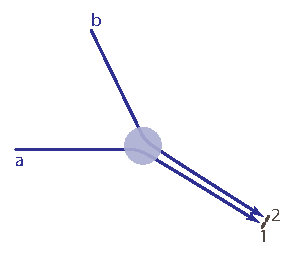
\includegraphics{fermions}
\end{center}
Since detectors 1 and 2 are approaching one another, we must have that
\begin{equation}
    |\braket{1}{a}\braket{2}{b}|^2 = |\braket{2}{a}\braket{1}{b}|^2.
\end{equation}
This does not imply, however, that $\braket{1}{a}\braket{2}{b} = \braket{2}{a}\braket{1}{b}$: the amplitudes could differ by a phase factor, so that interchanging the particles would yield
\[
    \braket{2}{a}\braket{1}{b} = e^{i\delta}\braket{1}{a}\braket{2}{b}.
\]
If we interchange the particles, and then interchange them again, we get
\[
    \braket{1}{a}\braket{2}{b} = e^{2i\delta}\braket{1}{a}\braket{2}{b};
\]
since swapping the particles twice just gets up back to the original situation, we must have that $e^{i\delta} = \pm 1$.

If there is no change of sign, i.e., $\braket{2}{a}\braket{1}{b} = \braket{1}{a}\braket{2}{b}$, then from equation~(\ref{e.scattering-quantum}) we have
\begin{equation}\label{e.boson}
    \mathcal{P}(\textrm{a or b in 1}) = 2|\braket{1}{a}\braket{2}{b}|^2 + 2|\braket{2}{a}\braket{1}{b}|^2.
\end{equation}
This is \emph{twice} the classical value: the probability of the particles entering the same state is enhanced.

In contrast, if $\braket{2}{a}\braket{1}{b} = -\braket{1}{a}\braket{2}{b}$, then equation~(\ref{e.scattering-quantum}) implies that
\begin{eqnarray}
\mathcal{P}(\textrm{a or b in 1}) &=& |\braket{1}{a}\braket{2}{b}| + |\braket{2}{a}\braket{1}{b}| \nonumber\\ 
    && - |\braket{1}{a}\braket{2}{b}| - |\braket{2}{a}\braket{1}{b}| \nonumber\\ 
    &=& 0.\label{e.fermion}
\end{eqnarray}
\begin{quote}\itshape
We cannot have 2 identical particles with the same momentum, position, and spin if their wavefunction changes sign when the particles are exchanged.
\end{quote}
Particles with integer spin (i.e., their angular momentum is an integer multiple of $\hbar$) have wavefunctions that do not change sign under exchange; these particles are said to obey \emph{Bose-Einstein statistics} and are called \emph{bosons}.  Particles with half-integer spin have wavefunctions that do change sign under exchange; these particles are said to obey \emph{Fermi-Dirac statistics} and are called \emph{fermions}.  Photons are bosons; electrons, protons, neutrons, and neutrinos are fermions.
\end{sidebar}

\newthought{To connect with the equation of state,} we begin by imagining a small volume containing $N$ electrons. Motivated by eq.~(\ref{e.heuristic-quantum-density}), we divide the phase space into cells,
\[
	\frac{\dif^{3}x\,\dif^{3}p}{h^{3}},
\]
and into each cell we place 2 electrons with opposing spins. We always add the electrons to the lowest open energy level, and repeat the process until we have added all $N$ electrons. This procedure is represented by the equation
\begin{equation}
	N = \frac{2}{h^{3}}\int_{V}\dif^{3}x\int_{0}^{\EF}\dif^{3}p
\end{equation}
In this equation $\EF$, the \emph{Fermi energy}, is the energy of the last electrons added and is the largest filled energy level.

If our volume is isotropic, then we can change variables: first, to spherical momentum coordinates, $\dif^{3}p = 4\pi p^{2}\,\dif p$; second, from $\dif p$ to $\dif\varepsilon$.  Since $p = \sqrt{2m\varepsilon}$, where $\varepsilon$ is the energy of a single electron,
\[
	\dif p = \sqrt{\frac{m}{2\varepsilon}}\,\dif \varepsilon;
\]
we can therefore change variables and integrate over $\varepsilon$ from $0$ to $\EF$ to obtain
\[
	N = \frac{8\pi}{h^{3}}V \int_{0}^{\EF} \sqrt{2}m^{3/2}\varepsilon^{1/2}\,\dif \varepsilon
	= \frac{8\pi}{3h^{3}} V (2m)^{3/2} \EF^{3/2}.
\]
Solving for the Fermi energy gives
\begin{equation}\label{e.fermi-energy}
	\EF = \frac{h^{2}}{2m}\left(\frac{3}{8\pi}\frac{N}{V}\right)^{2/3}.
\end{equation}
What is the total energy of our system? We again integrate over phase space, with each electron multiplied by its energy $\varepsilon$:
\begin{equation}\label{e.total-energy}
	E = \frac{8\pi}{h^{3}}V\int_{0}^{\EF}\sqrt{2}m^{3/2}\varepsilon^{3/2}\,\dif\varepsilon = \frac{8\pi}{5h^{3}}V(2m)^{3/2} \EF^{5/2}.
\end{equation}
Using eq.~(\ref{e.fermi-energy}) to substitute for $\EF$ in eq.~(\ref{e.total-energy}), we can find the energy per unit volume,
\[
	\frac{E}{V} = \frac{3}{5}\left(\frac{3}{8\pi}\right)^{2/3}\frac{h^{2}}{2m}n^{5/3} = \frac{3}{5} n \EF,
\]
where $n=N/V$ is the density of electrons.

Recall that for a non-relativistic gas the pressure is $P = (2/3)(E/V)$.  Hence the pressure of our electron gas is
\begin{equation}\label{e.pressure-electrons}
	P = \frac{2}{3}\frac{E}{V} = \frac{2}{5} n\EF
		= \frac{2}{5}\left(\frac{3}{8\pi}\right)^{2/3}\frac{h^{2}}{2m}n^{5/3}.
\end{equation}
Notice that the pressure is independent of the temperature.

The electrons, being more than 1000 times lighter than the nuclei, become degenerate first. Suppose our composition consists of species with charge $Z_{i}$ and mass number $A_{i}$. Then the number of electrons per unit volume\marginnote{assuming complete ionizaton} is
\[
	n_{e} = \sum_{i} n_{i} Z_{i} = \frac{\rho}{\mb}\sum_{i} X_{i}\frac{Z_{i}}{A_{i}}.
\]
By analogy with the mean molecular weight, we define an electron mean weight
\begin{equation}\label{e.electron-mean-weight}
\mu_{e} \equiv \left(\sum_{i}X_{i}\frac{Z_{i}}{A_{i}}\right)^{-1}
\end{equation}
so that $n_{e} = \rho/(\mb\mu_{e})$.

\begin{exercisebox}
\label{ex.degenerate-mass-radius}
Use equation~(\ref{e.electron-mean-weight}) in eq.~(\ref{e.pressure-electrons}) to express the pressure as a function of mass density $\rho$. The use the virial scalings for $P(M,R)$ and $\rho(M,R)$ to obtain a relation $R(M)$ for a degenerate object. \emph{Hint:} this may be easier to do in a Jupyter notebook.
\end{exercisebox}

As you found in exercise~\ref{ex.degenerate-mass-radius}, when the star becomes degenerate, there is a unique radius for a given mass and composition. This is in contrast to the non-degenerate case, for which a star of a given mass can have a wide range of possible radii depending on the internal temperature.

\section{Hydrogen burning}

\subsection{Hydrogen burning via pp reactions: the lower main sequence}

In a contracting pre-main sequence star, the reaction $\hydrogen[2]+p\to\gamma+\helium[3]$ proceeds rapidly owing to the small Coulomb barrier; in fact, this reaction can occur in objects as small as $\approx \val{12}{M_{\mathrm{Jupiter}}}$.  The small primordial abundance of deuterium, however, prevents this reaction from doing anything more than slowing contraction slightly.  The reaction $\pt +\pt$ is much slower, because there is no bound nucleus \helium[2]; the only possible way to form a nucleus is to have a weak interaction as well, giving the reaction $\pt+\pt\to e^{+}+\nu_{e}+\hydrogen[2]$.

The weak cross section goes roughly as $\sigma_{\mathrm{weak}} \sim \val{10^{-20}}{\barn}\left(E/\keV\right)$, so that
\[ \frac{\sigma_{\mathrm{weak}}}{\sigma_{\mathrm{nuc}}} \sim 10^{-23}\left(\frac{E}{\keV}\right). \]
The $S$-factor for the $\pt+\pt$ reaction is very small, and as a result the characteristic temperature for this reaction to occur is $\approx \val{\sci{1.5}{7}}{\K}$; at this temperature, the lifetime of a proton to forming deuterium via capture of another proton is about $\val{6}{\Giga\yr}$.  Once a deuterium nucleus is formed, it is immediately destroyed via $\hydrogen[2]+p\to\gamma+\helium[3]$. The nucleus \lithium[4] is unbound with a lifetime of $\val{10^{-22}}{\second}$; the nucleus \beryllium[6] is likewise unbound ($\tau \sim \val{\sci{5}{-21}}{\second}$). As a result, the next reaction that can occur is $\helium[3]+\helium[3]\to 2\pt+\helium$.  Despite having a much greater Gamow energy than $\pt + \pt$, this reaction still is much faster than $\pt+\pt$ owing to the small weak cross-section.

In addition to capturing another \helium[3], it is also possible that
\begin{eqnarray}
\helium[3] + \helium &\to& \beryllium[7] + \gamma\nonumber\\
 \beryllium[7] + e^{-} &\to& \lithium[7] +  \nu_{e}\qquad(\tau=\val{53}{\unitstyle{d}})\nonumber \\
 \lithium[7] + \pt &\to& 2\helium + \gamma;
 \end{eqnarray}
furthermore, at slightly higher temperatures \beryllium[7] can capture a proton instead of an electron, giving the third branch
\begin{eqnarray}
\beryllium[7] + \pt &\to& \boron[8] + \gamma\nonumber\\
\boron[8] &\to& \beryllium[8] + e^{+} + \nu_{e}\qquad(\tau = \val{770}{\milli\second})\nonumber\\
\beryllium[8] &\to& 2\helium\qquad(\tau= \val{10^{-16}}{\second}).
\end{eqnarray}
 The end result of these chains is the conversion of hydrogen to helium, although the amount of energy carried away by neutrinos differs from one chain to the next.

\subsection[The CNO cycle]{Hydrogen burning via the CNO cycle: the upper main sequence}

As we saw in the previous section, the smallness of the $\pt+\pt$ cross-section means that captures onto heavier nuclei can be competitive at stellar temperatures.  Let's get a rough estimate of how charged a nucleus can be before the Coulomb barrier makes the reaction slower than $\pt+\pt$.  Assuming $A = 2Z$, and taking the $S$-factor for $\pt+\pt$ to be $10^{-22}$ times smaller that that for $\pt + \mathrm{^{A}Z}$ gives us the rough equation
\[ 10^{-22}\exp\left(-\frac{33.81}{T_{6}^{1/3}}\right) \approx \exp\left(-\frac{41.47 Z^{2/3}}{T_{6}^{1/3}}\right), \]
where the factors in the exponentials come from the peak energy for the reaction (see the handout on nuclear burning), and $T_{6}\equiv (T/\val{10^{6}}{\K})$.  Solving for $Z$, we see that at $T_{6} = 10$, proton captures onto \carbon\ have a comparable cross-section to $\pt + \pt$; at $T_{6} = 20$, proton captures onto \oxygen\ have a comparable cross-section.

Thus at temperatures slightly greater than that in the solar center, the following catalytic cycle becomes possible.
\begin{center}
\begin{tabular}{rr}
reaction & $\log[(\tau/\yr) \times (\rho X_{H}/\val{100}{\grampercc})]$\\
\hline
$\carbon(\mathbf{p},\gamma)\nitrogen[13]$ & 3.82\\
$\nitrogen[13](,e^{+}\nu_{e})\carbon[13]$ & $\tau=\val{870}{\second}$\\
$\carbon[13](\mathbf{p},\gamma)\nitrogen[14]$ & 3.21\\
$\nitrogen[14](\mathbf{p},\gamma)\oxygen[15]$ & 5.89 \\
$\oxygen[15](,e^{+}\nu_{e})\nitrogen[15]$ & $\tau = \val{178}{\second}$\\
$\nitrogen[15](\mathbf{p},\mathbf{^4He})\carbon$ & 1.50 \\
\hline
\end{tabular}
\end{center}
As indicated by the boldfaced symbols, this cycle takes in 4 protons and releases 1 helium nucleus.
The reaction timescales are evaluated at a temperature of $\val{20}{\Mega\K}$.
The reaction $\nitrogen+\pt\to\gamma+\oxygen[15]$ is by far the slowest step in the cycle; as a result, all of the CNO elements are quickly converted into \nitrogen\ in the stellar core, and this reaction controls the rate of heating.  At $T = \val{\sci{2}{7}}{\K}$, $\dif \ln \varepsilon_{\mathrm{CNO}}/\dif\ln T = 18$; in contrast the $\pt+\pt$ reaction has a temperature exponent of only 4.5.

The strong temperature dependence of the CNO burning has two effects on the structure of the star.  First, it makes the central temperature nearly constant over a wide range of stellar masses for $M > \val{1}{\Msun}$. A constant central temperature implies, via the virial theorem, that $R \propto M$ on the upper main sequence.  A second consequence is that nearly all of the star's luminosity is generated in a small mass about the stellar center.  This drives the cores of massive stars to be convective.

\section{Summary}

This convective zone changes the structure of the star, so that $L\sim M^{3.5}$ rather than the $M^{3}$ scaling we derived earlier.  It also means the star can burn more of the hydrogen in its interior.  The hotter $\Teff$ means, however, that the opacity is less strong in the surface layers of upper main sequence stars, and so the outer layers are radiative.  Table~\ref{t.MS-characteristics} gives a summary of the properties of main sequence stars.
\begin{margintable}[-6\baselineskip]
\caption{\label{t.MS-characteristics} Characteristics of main-sequence stars}
\centering
\begin{tabular}{lll}
characteristic & $M\lesssim\Msun$ & $M\gtrsim\Msun$\\
\hline
hydrogen burning & pp & CNO\\
core & radiative  & convective\\
envelope & convective & radiative\\
\end{tabular}
\end{margintable}
